\newpage
\part{开发与测试}

在开发中,我采用了成熟的开发工具,包括编译工具、编辑工具来加快开发速度,保证代码质量;我也借助\lstinline{cmocka}库对YaDNS的主要算法与数据结构的实现进行了单元测试,保证代码质量,保证算法逻辑的正确性。

\section{开发环境与构建环境}

软件开发使用的工具与环境如下所示:
\begin{enumerate}
  \item macOS Catalina 10.15.6
  \item fish (friendly interactive shell), version 3.1.2
  \item iTerm 2, 3.3.12
  \item CMake 3.17.2
  \item Ninja 1.10.0
  \item Conan 1.28.1
  \item CLion 2020.2.1
  \item Visual Studio Code 1.48.2
\end{enumerate}

具体地,在开发中我使用的主力集成开发环境为CLion,CLion提供了成熟的代码高亮、语法提示、纠错与警告等功能,并提供了许多方便的代码补全行为,也具有方便的快捷键与将为好用的 Vim 模式,为提高开发效率提供了莫大的帮助。

而在构建方面,我使用CMake作为构建系统,一方面因为他的成熟与好用,另一方面因为它是与CLion最为契合的构建方式。而使用Ninja作为构建器,执行CMake生成的构建规则。使用Conan来进行依赖管理,保证了构建的可移植与可复现。

\section{单元测试}

对于YaDNS中使用到的主要数据结构以及算法,我借助 \lstinline{cmocka} 进行了单元测试,来保证其正确性。测试的部分主要包括:对本地记录文件的解析与读取、队列、\lstinline{Trie}树。

\paragraph{本地记录文件的解析} 这一部分主要测试了对记录文件中域名、IP地址的读取与解析。保证了主要函数功能的正确性。除此以外,也对存储记录的数据结构的创建与销毁进行了测试。

\paragraph{队列} 在YaDNS的查询池、请求池、连接池中都使用到了队列的数据结构来进行池中资源的维护与管理。单元测试覆盖了队列的入队、出队等主要操作,以及对队列空、满情况的判断,对元素是否在队列中的判断等等。

\paragraph{\lstinline{Trie} 树} DNS响应缓存中使用了 \lstinline{Trie} 树来将域名映射到对应的资源记录。单元测试对\lstinline{Trie} 树的插入、查找、销毁以及垃圾回收等功能进行了测试。

YaDNS对于这三个部分共添加了23个单元测试。在开发过程中,通过测试可以保证代码质量,减少显然的错误,降低调试成本。大大提升开发效率。图 \ref{fig:unit-tests} 中是YaDNS通过23个单元测试的运行截图。

\begin{figure}[h]
  \centering
  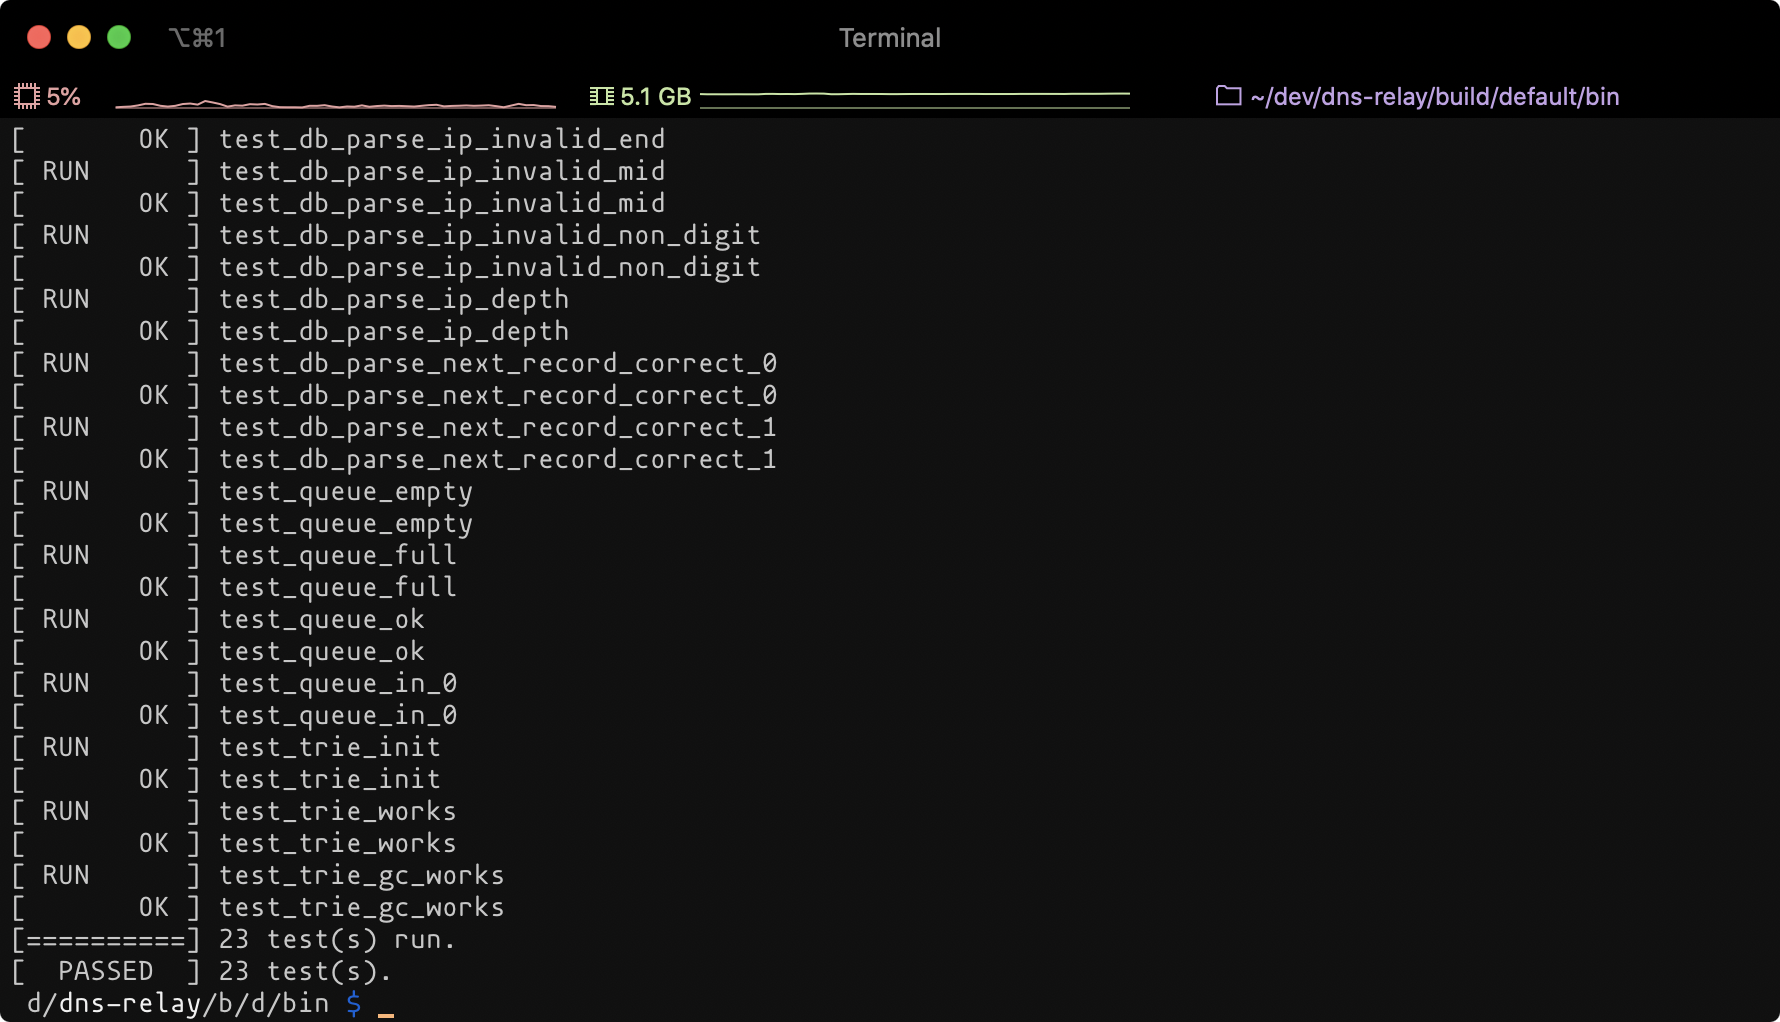
\includegraphics[width=0.7\textwidth]{figures/unit_tests}
  \caption{单元测试运行结果}
  \label{fig:unit-tests}
\end{figure}

